\documentclass[ngerman,hyperref={pdfpagelabels=false}]{beamer}

% -----------------------------------------------------------------------------

\graphicspath{{images/}}
\usepackage{graphics}
\usepackage{multimedia}
% -----------------------------------------------------------------------------

\usetheme{KIT}

\setbeamercovered{transparent}
%\setbeamertemplate{enumerate items}[ball]

\newenvironment<>{KITtestblock}[2][]
{\begin{KITcolblock}<#1>{#2}{KITblack15}{KITblack50}}
{\end{KITcolblock}}

\usepackage[ngerman,english]{babel}
\usepackage{animate}
\usepackage[utf8]{inputenc}
\usepackage[TS1,T1]{fontenc}
\usepackage{array}
\usepackage{multicol}
\usepackage[absolute,overlay]{textpos}
\usepackage{beamerKITdefs}
\usepackage[ruled,vlined,linesnumbered,norelsize]{algorithm2e}

\pdfpageattr {/Group << /S /Transparency /I true /CS /DeviceRGB>>}	%required to prevent color shifting withd transparent images


\title{SAT Solving with distributed local search}
\subtitle{Guangping Li -- \textit{uzdif@student.kit.edu}}

\author[Guangping Li]{Guangping Li}
\institute{Institute of Theoretical informatics, Algorithmics II}

\TitleImage[width=\titleimagewd,height=\titleimageht]{titel}

\KITinstitute{Institute of Theoretical informatics}
\KITfaculty{KIT Department of Informatics}

% -----------------------------------------------------------------------------

\begin{document}
\setlength\textheight{7cm} %required for correct vertical alignment, if [t] is not used as documentclass parameter


% title frame
\begin{frame}
  \maketitle
\end{frame}


% intro
\section{Presentation}
\begin{frame}
  \frametitle{Outline}

\heading{ \color<beamer:2>{red}{Propositional Satisfiability Problem (\emph{\textbf{SAT}})}}
  \begin{itemize}
  \item Notations
  \item Local search in SAT problem
  \end{itemize}
\heading{Solving SAT by \emph{swpSolver}}
  \begin{itemize}
  \item Basic scheme
  \item Our improvements
  \end{itemize}
\heading{Our Parallel SAT-solver}
  \begin{itemize}
  \item The pure portfolio approach
  \item Failures
  \item Initialization with a guide of formula partitioning
  \end{itemize}
\heading{Conclusion}
  
\end{frame}


% blocks
\begin{frame}
	\frametitle{Propositional Satisfiability Problem}

	\begin{KITalertblock}{Notations}
	\begin{itemize}
	\item propositional variable: variable with two possible logical values  \textit{true} or  \textit{false}
	\item literal: an atomic formula either be a positive literal $v$ or a negative literal $\bar{v}$.\\
	\item clause: disjunction of literals.
	\item CNF-formula: conjunction of clauses
	\item assignment: $V\rightarrow \{true {, }\; false\}$ 
	\item SAT problem: to determine whether a given formula is satisfiable or not  \\
	\end{itemize}
	\end{KITalertblock}
\end{frame}
\begin{frame}
	\frametitle{Here is an example of SAT problem:}
\begin{center}
\begin{table}[H]
\begin{tabular}{l}
$F = (v_1 \lor \bar{v_3}) \land (v_2 \lor v_1 \lor \bar{v_1})$\\	
$Vars(F) = \{v_1, v_2, v_3\}$\\
$numV(F) = |Vars(F)| = 3$\\
$Lits(F) = \{v_1, \bar{v_1}, v_2, v_3, \bar{v_3}\}$\\
$Cls(F) = \{C_1, C_2\}$\\
$numC(F) = |Cls| = 2$\\ 
$C_1 = \{v_1, \bar{v_3}\}$\\
$C_2 = \{v_2, v_3, \bar{v_1}\}$\\
\\
$A(v_1)$ = $true$, $A(v_2)$ = $false$, $A(v_3)$ = $true$, \\
$A$  is an assignment satisfying $F$.\\
\\
$\hat{A}(v_1)$ = $true$, $\hat{A}(v_2)$ = $false$, $\hat{A}(v_3)$ = $false$, \\
$\hat{A}$  is an assignment with conflict in $C_2$.\\
\end{tabular}
\end{table}
\end{center}
\end{frame}
\begin{frame}
	\frametitle{ Local search in SAT problem}
		\begin{KITexampleblock}{Local Search}
	  \begin{itemize}
	\item an instance $I$ of a hard combinational Problem $P$
	\item a set of solutions $S(I)$
	\item an object function (score or cost) $\Gamma$ 
	\item to find the solution with minimum cost by applying local changes.
\end{itemize}
	\end{KITexampleblock}
\begin{algorithm}[H]
\SetKwInOut{Input}{input}
\SetKwInOut{Output}{output}
\SetKwInOut{Parameter}{parameter}
 \Input{A CNF Formula F}
 \Parameter{$Timeout$}
 \Output{a satisfying assignment $A$}
  $A \leftarrow$ random generated assignment  $A$\\
 \While {$( \exists$ unsatisfied clause $ \land$ Timeout does not occur$)$}{
  $c \leftarrow$ random selected  unsatisfied clause \\
  $x \leftarrow pickVar(A,c)$\\
  $A \leftarrow flip(A,x)$\\
 }
 \caption{Focused Local Search}
\end{algorithm} 
\end{frame}
\begin{frame}
	\frametitle{ Local search in SAT problem}
		\begin{KITexampleblock}{Stochastic Local Search (SLS)}
\begin{itemize}
\item use the probability distribution of the scores of candidate solutions 
\item the more advantageous a move is, the higher is the probability of choosing that move
\end{itemize}
\end{KITexampleblock}
\begin{algorithm}[H]
\SetKwInOut{Input}{input}
\SetKwInOut{Output}{output}
\SetKwInOut{Parameter}{parameter}
 \Input{current assignment $A$, unsatisfied clause $c$}
 \Output{a variable $x$ in $c$ to be flipped}
\For{$v$ in $c$}{
  Evaluate $v$ with function $\Gamma(A,v)$\;
 }
  $x \leftarrow$ randomly selected  variable $v$ in $c$ with probability $p(v) =\frac{\Gamma(A,v)}{\sum_{u \in c}\Gamma(A,u)}$ 
 \caption{PickVar in \emph{probSAT}}
 \end{algorithm} 
\end{frame}
\begin{frame}
	\frametitle{ Local search in SAT problem}
		\begin{KITexampleblock}{Random walk in local search}
		\begin{itemize}
         \item originally introduced in 1994
         \item By introducing ``uphill noises'', the walkSAT combines greedy local search and random walk.
\end{itemize}
\end{KITexampleblock}
\begin{algorithm}[H]
\SetKwInOut{Input}{input}
\SetKwInOut{Output}{output}
\SetKwInOut{Parameter}{parameter}
 \Input{current assignment $A$, unsatisfied clause $c$}
 \Parameter{probability $p$}
 \Output{a variable $x$ in $c$ to be flipped}
\For{$v$ in $c$}{
  Evaluate $v$ with function $\Gamma(A,v)$\;
 }
  with probability $p$: $x \leftarrow$   $v$ with maximum $\Gamma(A,v)$ \;
  with probability $1-p$:  $x \leftarrow$  randomly selected $v$ in $c$. 
 \caption{PickVar in walkSAT}
\end{algorithm}  
\end{frame}
\begin{frame}
  \frametitle{Outline}
\heading{Propositional Satisfiability Problem (\emph{\textbf{SAT}})}
  \begin{itemize}
  \item Notations
  \item Local search in SAT problem
  \end{itemize}
\heading{\color<beamer:1>{red}{Solving SAT by \emph{swpSolver}}}
  \begin{itemize}
  \item Basic scheme
  \item Our improvements
  \end{itemize}
\heading{Our Parallel SAT-solver}
  \begin{itemize}
  \item The pure portfolio approach
   \item Failures
  \item Initialization with a guide of formula partitioning
  \end{itemize}
\heading{Conclusion}
\end{frame}
% blocks continued
\begin{frame}
	\frametitle{Solving SAT by \emph{swpSolver}}
	\framesubtitle{Basic scheme}
\begin{algorithm}[H]
\SetKwInOut{Input}{input}
\SetKwInOut{Output}{output}
\SetKwInOut{Parameter}{parameter}
 \Input{A CNF Formula F}
 \Parameter{$Timeout$}
 \Output{a satisfying assignment $A$}
  $A \leftarrow initAssign(F)$ \;
 \While {$( \exists$ unsatisfied clause $ \land$ Timeout does not occur$)$}{
  $c \leftarrow pickCla(A)$ \;
  $x \leftarrow pickVar(A,c)$\;
  $A \leftarrow flip(A,x)$\;
 }
 \caption{Our Local Search}
\end{algorithm}
\end{frame}
\begin{frame}
\frametitle{Evaluation}
\begin{itemize}
\item 180 instances (\emph{UNIF}) in random benchmark categories in SAT competition 2017
\item All the clause have the same length $k$ in a \emph{UNIF} problem file.
\item to construct one clause, $k$ literals are randomly chosen from the $2n$ possible literals
\item At least $60$ ( $33\%$ ) problems form our $180$ benchmark collections are unsatisfiable.
\item Each experiment is repeated three times.
\item PAR-2 runtime for a whole $k$SAT set
\end{itemize}
\end{frame}
\begin{frame}
	\frametitle{initAssign(F)}	
	\begin{itemize}
\item \emph{RandomInit}: build a complete assignment randomly
\item \emph{BiasInit}: assign \emph{true} to a variable if the number of occurrences of its positive literal is larger than that of its negative literal.  
\item \emph{Bias-RandomInit}: assign \emph{true} to variable $v_i$ with probability $\frac{posOccurences[i]}{posOccurences[i]+negOccurences[i]}$.
\end{itemize} 
\end{frame}
\begin{frame}
	\frametitle{initAssign(F)}	
\begin{table}[H]
\label{tab:com}
%\begin{minipage}{\textwidth}                                                                                         
\begin{center}
    \begin{tabular}{|l|l|l|l|p{1cm}|}
\hline 
    k &\emph{RandomInit}&\emph{BiasInit}&\emph{Bias-RandomInit} \\ \hline
	3&9221.9 &9157.76 &\textbf{9078.27} \\ 
	&\textbf{55} &54 & \textbf{55} \\ \hline
	5&7143.9&\textbf{4351.09}&4582.54\\ 
	&82 &\textbf{87} &\textbf{87}\\ \hline
	7&6238.51&\textbf{5421.9}& 6310.7\\
	&60 & 60 & 60 \\ \hline
	
\end{tabular}
\end{center}
%\end{minipage}
\end{table}
\begin{itemize}
\item 3SAT: RandomInit
\item 5SAT and 7SAT: BiasInit
\end{itemize} 
\end{frame}

\begin{frame}
\frametitle{pickVar(A,c)}
\begin{itemize}
\item combine the random walk and stochastic selection
\item pick greedy flips with zero breakcounts with a certain probability $p$.
\item use the \emph{SLS} with probability ($1-p$) 
\end{itemize}
\begin{algorithm}[H]
\SetKwInOut{Input}{input}
\SetKwInOut{Output}{output}
\SetKwInOut{Parameter}{parameter}
 \Input{current assignment $A$, unsatisfied clause $c$}
 \Parameter{probability $p$}
 \Output{a variable $x$ in $c$ to be flipped}
 \emph{greedyVs} $\leftarrow$ $\emptyset$\;
\For{all $v$ in $c$}{
   \If{$($break(A,v)= 0 $)$}{
	\emph{greedyVs} = \emph{greedyVs} +  $\{v\}$    
   }
 }
  with probability $p$: $x \leftarrow$ randomly selected variable $v \in$ \emph{greedyVs} \;
  with probability ($1-p$):   $x \leftarrow$ randomly selected  variable $v$ in $c$ with probability $\frac{\Gamma(A,v)}{\sum_{u \in c}\Gamma(A,u)}$
\caption{Our pickVar}
\end{algorithm}  
\end{frame}

\begin{frame}
\frametitle{Variant 1: Walk}
\begin{itemize}
\item statistic list $S$: how many times each variable is chosen for flipping
\item The candidate with the small statistic value will be chosen.
\item $p = \alpha \times \frac{s(randomV)}{s(greedyV)+s(randomV)}$
\item Getting the random literals using stochastic process consumes the most runtime.
\end{itemize}
\end{frame}
\begin{frame}
\frametitle{Variant 2: GreedyBreak}
\begin{itemize}
\item  \emph{permitted greedy literal}: literal with zero breakcount and its statistic value is under a certain threshold $t$
\item choose a permitted greedy literal randomly for flipping. 
\item if no permitted greedy literal exists, we pick a literal using \emph{SLS} heuristic.
\item 1st approach \emph{Average}: $t = \alpha \times \frac{numF}{numV}$
\item 2nd approach \emph{Random-Flip}: $t =\alpha \times r$  with $r \in [0, numF]$.
\end{itemize}
\end{frame}
\begin{frame}
\frametitle{PickVar(A,c) with simulated annealing}
\begin{KITexampleblock}{Simulated Annealing}
\begin{itemize}
\item proposed by Kirkpatrick, Gelatt, and Vecchi.
\item guide local search with a controlling parameter \emph{\textbf{temperature}}. 
\item The temperature varies according to the score of the current situation. 
\item Higher temperature allows uphill moves with higher probability. 
\end{itemize}
\end{KITexampleblock}
\begin{itemize}
\item Walk: $p = \alpha \times \frac{s(randomV)}{s(greedyV)+s(randomV)}$
\item Average: $t = \alpha \times \frac{numF}{numV}$
\item Random-Flip: $t =\alpha \times r$  with $r \in [0, numF]$.
\item $\alpha = \tau \times (c_b)^{-q(A)}$
\item two variants of  $q(A)$:
\begin{itemize}
\item $q_{global}(A) =unsatN(A)$
\item $q_{local}(A) =|\{ v| v \in  c \land break(v) = 0\}|$
\end{itemize}
\end{itemize}
\end{frame}

\begin{frame}
\frametitle{Evaluation}
\framesubtitle{pickVar}
\begin{itemize}
\item probSAT: 
\begin{itemize}
\item implemented by the authors of the original paper
\item non-incremental approach to the 3SAT problems and incremental method for 5SAT and 7SAT
\end{itemize}
\item yalSAT:
\begin{itemize}
\item  the third version of yalSAT submitted to the 2017 SAT competition
\item  uses a variant of \emph{probSAT} randomly in the restart of a searchround
\end{itemize}
\end{itemize}
    \begin{tabular}{|l|l|l|l|l|p{2.5cm}|}
\hline 
    k &\emph{probSAT}&\emph{yalSAT}&\emph{Walk}&\emph{Average}&\emph{Random-Flip} \\ \hline      
    3 &9221.9&17062.35&7430.12&\textbf{6161.11} &7308.01\\ 
    &55&41&57&\textbf{61}&58\\ \hline
    5& 7143.9&5676.63&3330.61&\textbf{2939.74}&4003.06\\ 
    &82&85&\textbf{89}&\textbf{89}&88\\ \hline
    7& 6238.51&10063.4&5409.67&\textbf{3829.95}&4903.61\\
    &60&54&61&\textbf{65}&60\\ \hline
\end{tabular}
\end{frame}

\begin{frame}
\frametitle{Evaluation}
\framesubtitle{pickVar}
  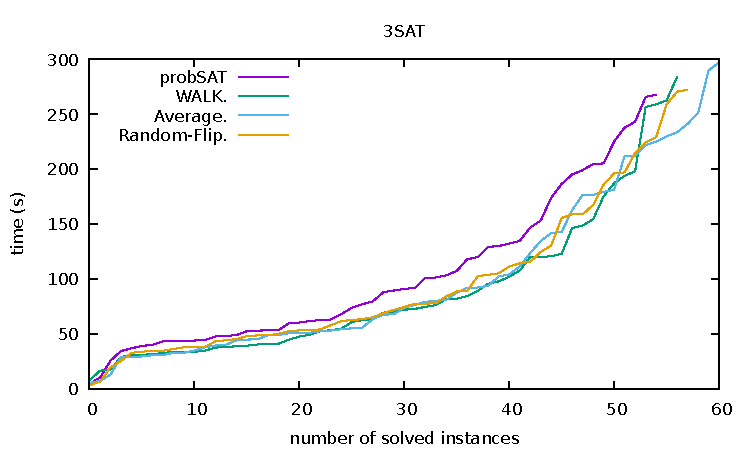
\includegraphics[scale = 0.9]{DATA/K3/e4.pdf}
\end{frame}
\begin{frame}
\frametitle{Evaluation}
\framesubtitle{pickVar}
    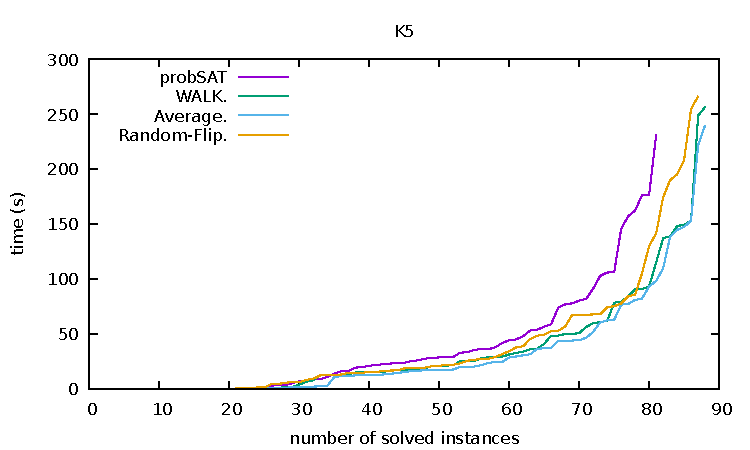
\includegraphics[scale = 0.9]{DATA/K5/e4.pdf}
\end{frame}
\begin{frame}
\frametitle{Evaluation}
\framesubtitle{pickVar}
  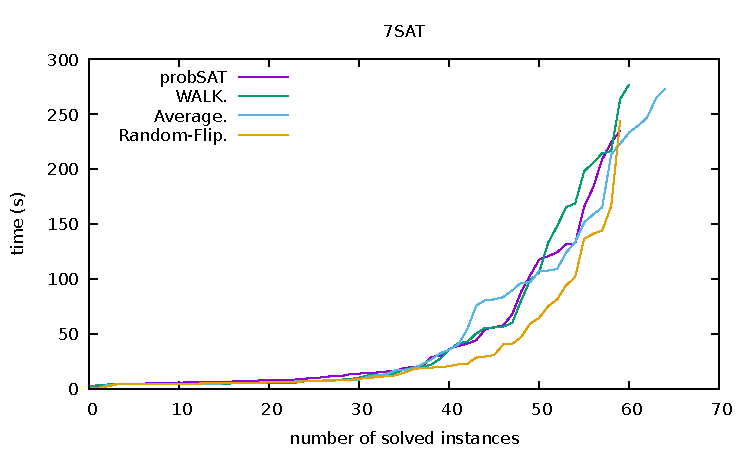
\includegraphics[scale = 0.9]{DATA/K7/e4.pdf}
\end{frame}

\begin{frame}
\frametitle{Evaluation}
\framesubtitle{swpSolver}
  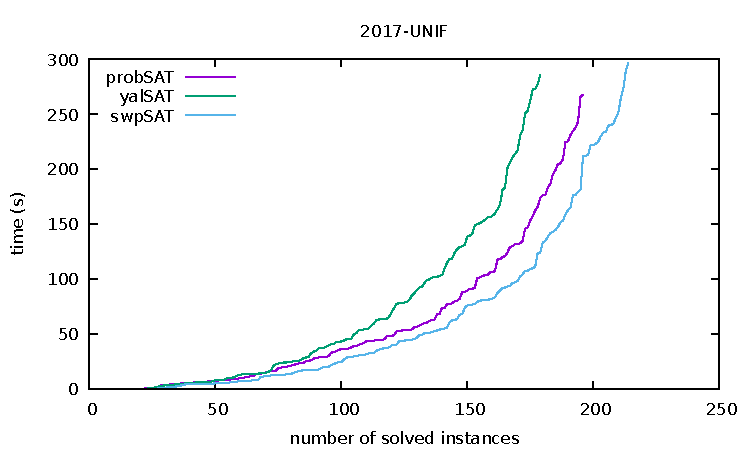
\includegraphics[scale = 0.9]{DATA/UNIF/e5.pdf}
\end{frame}
\begin{frame}
  \frametitle{Outline}

\heading{Propositional Satisfiability Problem (\emph{\textbf{SAT}})}
  \begin{itemize}
  \item Notations
  \item Local search in SAT problem
  \end{itemize}
\heading{Solving SAT by \emph{swpSolver}}
  \begin{itemize}
  \item Basic scheme
  \item Our improvements
  \end{itemize}
\heading{\color<beamer:1>{red}{Our Parallel SAT-solver}}
  \begin{itemize}
  \item The pure portfolio approach
  \item Failures
  \item Initialization with a guide of formula partitioning
  \end{itemize}
\heading{Conclusion}
  
\end{frame}
\begin{frame}
	\frametitle{The pure portfolio approach}
\begin{itemize}
\item random generator affects the performance. 
\item the agents run the \emph{swpSAT} with different random generation policies. 
\end{itemize}
\begin{table}[h!]
\begin{center}
    \begin{tabular}{|l|l|l|l|l|p{1cm}|}
\hline 
$rand()$&$minstd\_rand$&$mt19937$\\ \hline
$mt19937\_64$&$ranlux24\_base$&$ranlux48\_base$\\ \hline
$ranlux24$&$ranlux48$&$knuth\_b$\\ \hline
$default\_random\_engine$&$minstd\_rand0$&-\\ \hline
\end{tabular}
\end{center}
\end{table} 

   \begin{table}[H]
   \label{tab:UNIF}
%\begin{minipage}{\textwidth}                                                                                         
\begin{center}
    \begin{tabular}{|l|l|l|l|l|p{3cm}|}
\hline 

    k &\emph{swpSAT}&\emph{pure portfolio}&Speedup&Efficiency\\ \hline      
    3 &12971.3&7426.9 & 1.75& 0.16 \\ 
    &59&69&&\\ \hline
    5&8339.98&5185.75&1.61&0.14\\ 
    &89&94&&\\ \hline
    7&13406.26&2853.81&4.70&0.43\\
    &66&83&&\\ \hline
	
\end{tabular}
\end{center}
\end{table}
\end{frame}
\begin{frame}
  \frametitle{Evaluation}
	\framesubtitle{ benchmark \emph{COMBINE}}
	\begin{itemize}
	\item formula partitioning by a relatively balanced partitioning with small intersection
	\item combine two \emph{UNIF} benchmark instances
	\item build the intersection based on a randomly chosen satisfying assignment
\begin{itemize}
\item \emph{BIG}: \emph{COMBINE} problems with big intersection ($\frac{numCI}{numC} > 1\%$)
\item \emph{SMALL}: \emph{COMBINE} problems with big intersection ($\frac{numCI}{numC} < 1\%$)
\end{itemize}
\end{itemize}
\end{frame}
\begin{frame}
	\frametitle{Failures}
    \framesubtitle{2nd Approach: Solver with formula partitioning}
\begin{figure}[H]
\begin{center}
  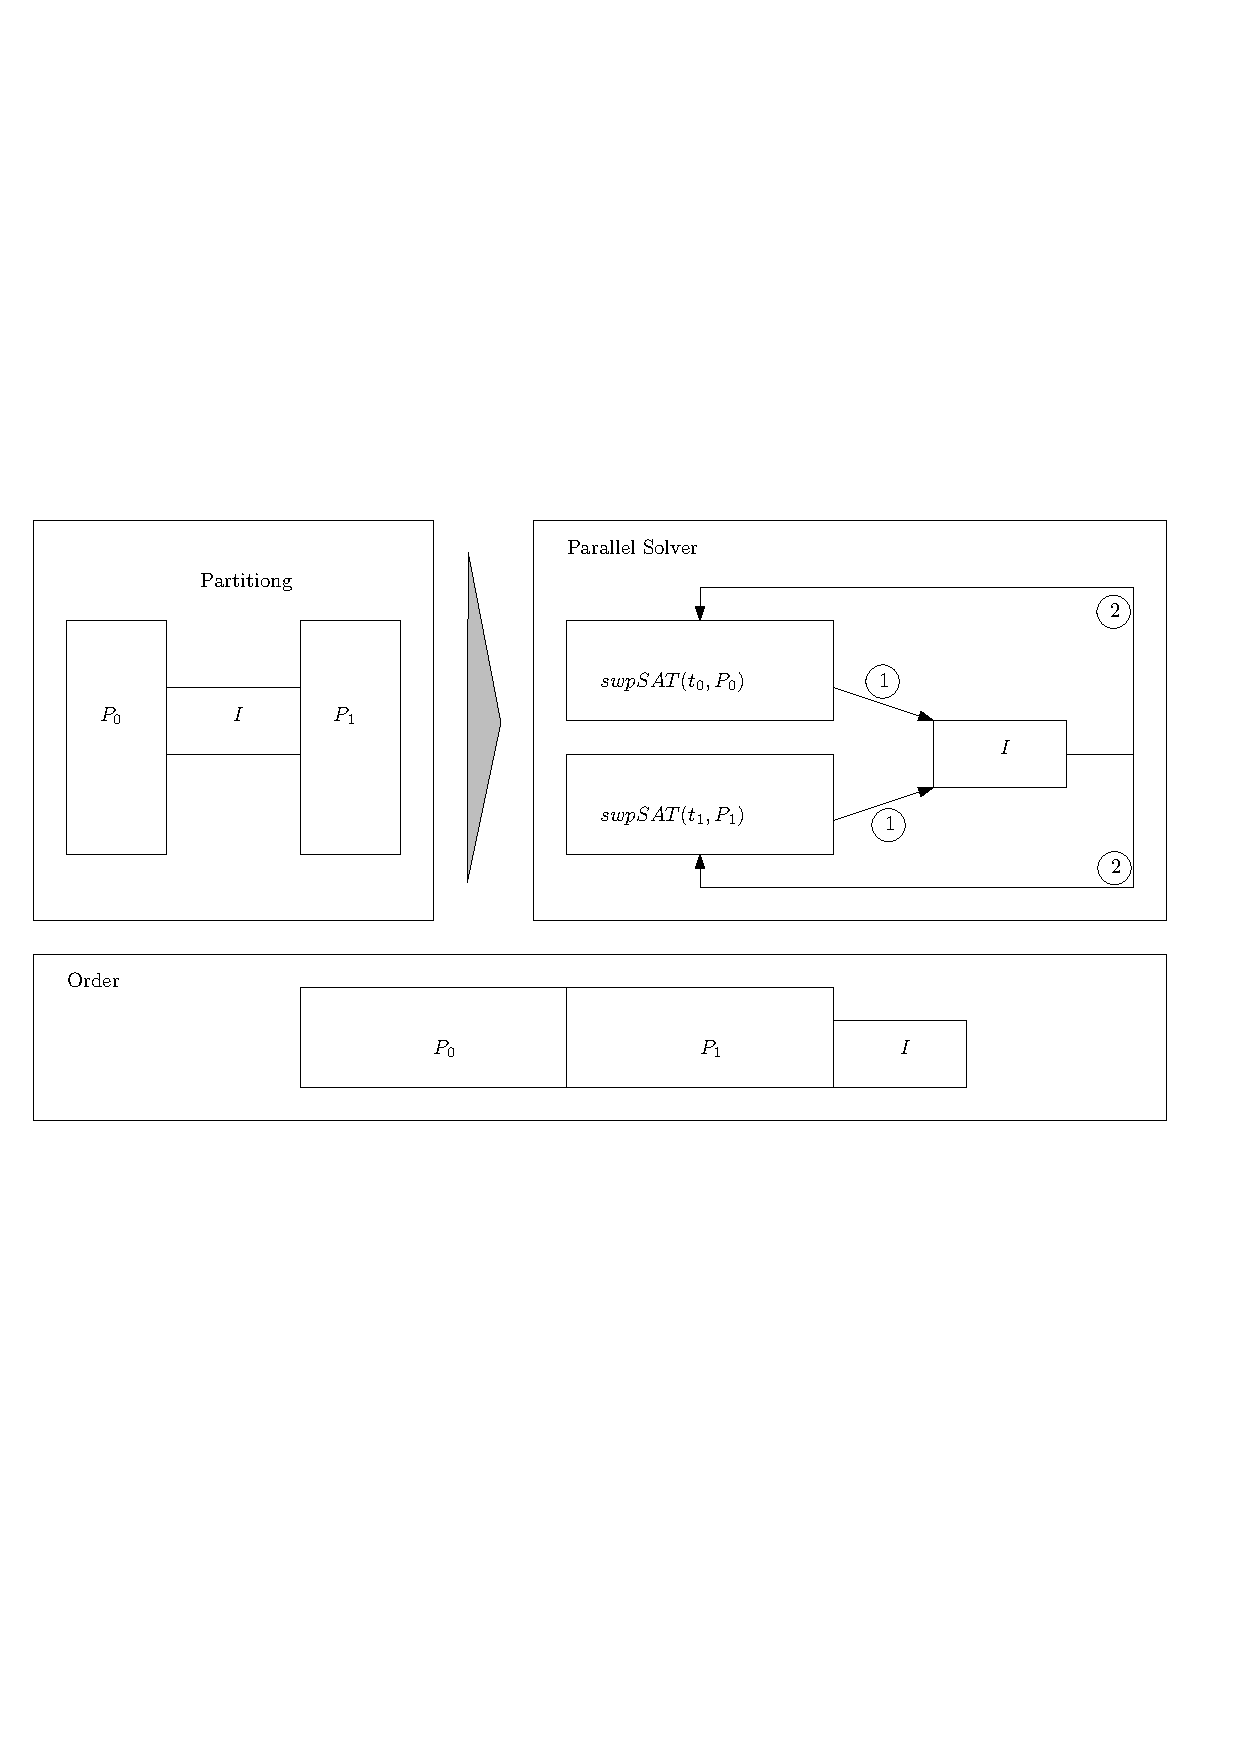
\includegraphics[scale = 0.6]{ipe/aproach2.pdf}
  \end{center}
  \label{a2}
  \end{figure}
\end{frame}

\begin{frame}
	\frametitle{Failures}
    \framesubtitle{3nd Approach: Solver with combination of sub-assignments}
\begin{figure}[H]
\begin{center}
  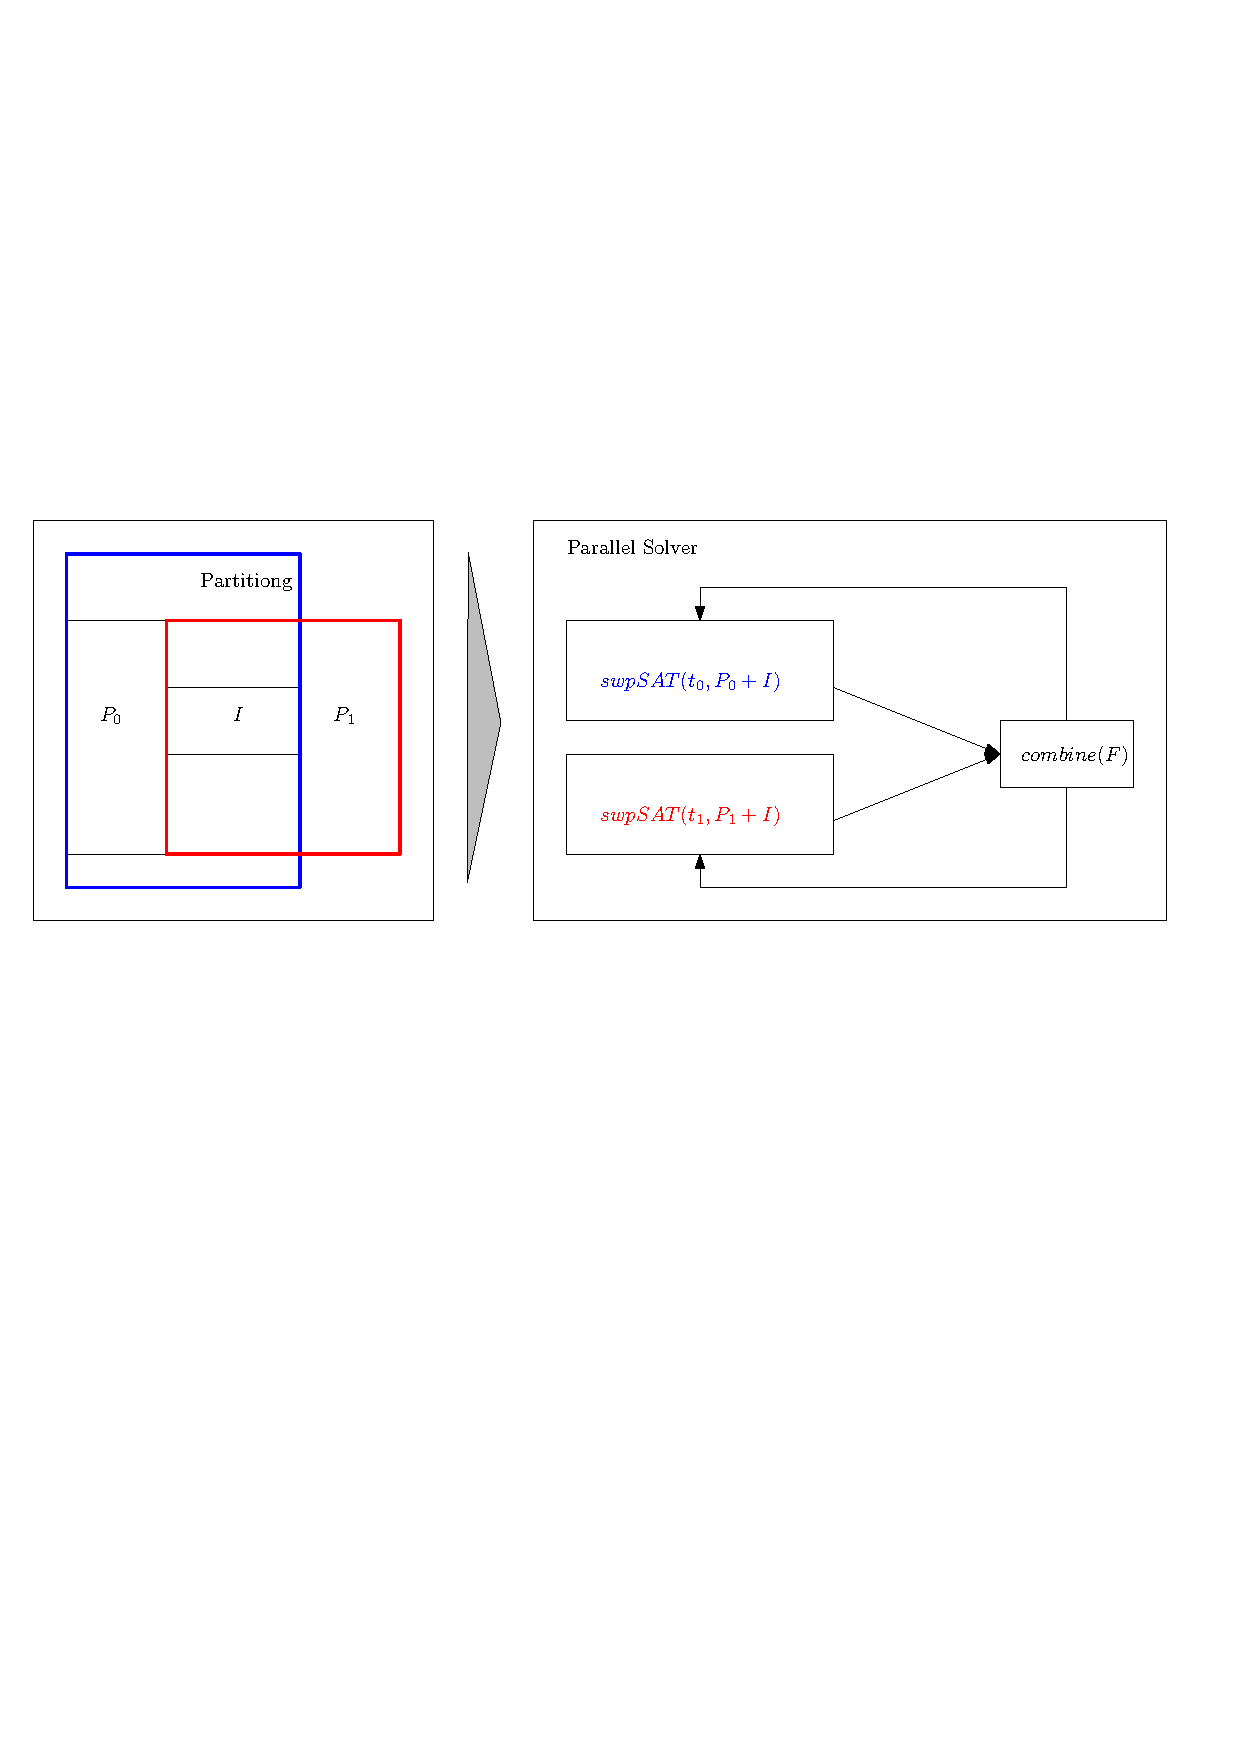
\includegraphics[scale = 0.61]{ipe/aproach3.pdf}
  \end{center}
  \label{a2}
  \end{figure}
\end{frame}

\begin{frame}
	\frametitle{Our Parallel GCP-solver}
    \framesubtitle{4th Approach: Initialization with formula partitioning (\emph{FineInit})}
\begin{itemize}
\item The formula partitioning information is only used to get an initial solution. 
\item The statistic information shared among the agents encourages the further search to flip non-critical variables in clauses.
\item The candidate with the smallest statistic value will be chosen in the next step.  
\item The agents use one common statistic matrix.\\
\end{itemize}
\end{frame}
\begin{frame}
  \frametitle{Evaluation}
	\framesubtitle{ benchmark \emph{COMBINE}-\emph{BIG}}
  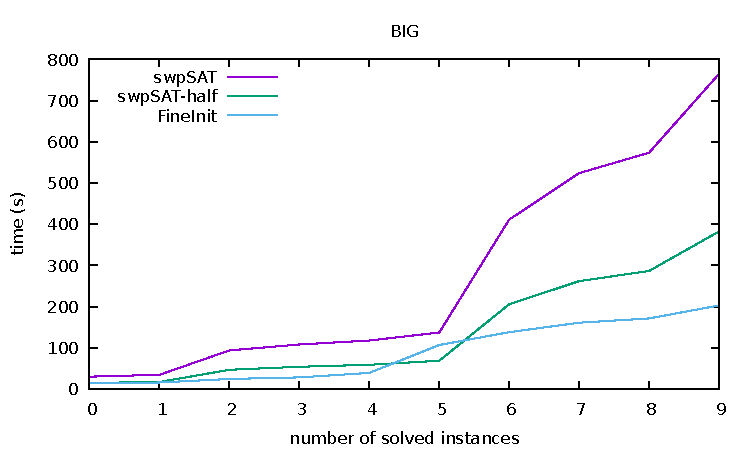
\includegraphics[scale = 0.9]{DATA/BIG/a4.pdf}
\end{frame}
\begin{frame}
  \frametitle{Evaluation}
	\framesubtitle{ benchmark \emph{COMBINE}-\emph{SMALL}}
    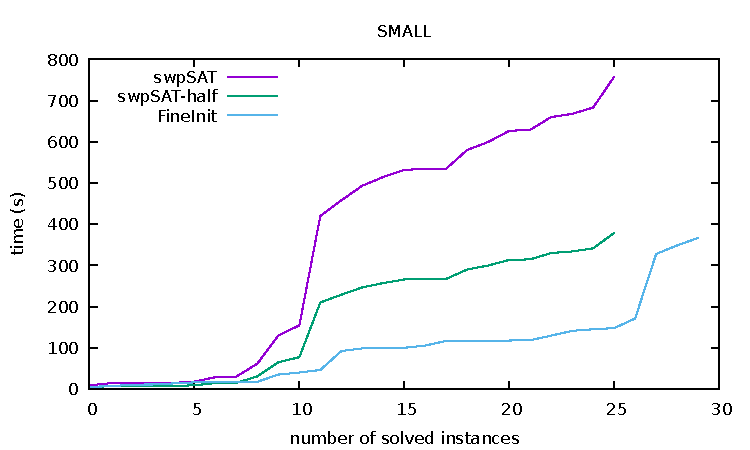
\includegraphics[scale = 0.9]{DATA/SMALL/a4.pdf}
\end{frame}
\begin{frame}
\frametitle{Our parallel solver}
\begin{itemize}
\item uses \emph{FineInit} as initialization
\item tries different search paths with  pure portfolio approach 
\end{itemize}
\begin{algorithm}[H]
\SetKwInOut{Input}{input}
\SetKwInOut{Output}{output}
\SetKwInOut{Parameter}{parameter}
 \Input{A CNF Formula $F$, number of Processors $n_p$ }
  $A \leftarrow initAssign(F)$\;
 \ForEach{$(Processor_t$ for $t \in \{1, .., n_p\})$}{
    $A_t \leftarrow A$\;
     $i\leftarrow t\%2$\;
	swpSAT($P_i$)\;
	swpSAT($P_{1-i}$) \;
 \While {$(!sat$  $ \land$ !Timeout$)$}{
     $A_t \leftarrow A$\;
 	 swpSAT($F$)\;
 	 $sat\leftarrow true$\;
 }
 }
\end{algorithm}  
\end{frame}
\begin{frame}
  \frametitle{Evaluation}
	\framesubtitle{ benchmark UNIF}
	\begin{itemize}
	\item separate the vertices according their indices in two partition sets
	\item All vertices $v_i$ with $i <\frac{numV}{2}$  belong to $P_0$.
	\item The rest vertices belong to $P_1$.
	\end{itemize}
\begin{table}[H]
%begin{minipage}{\textwidth}                                                                                         
\begin{center}
    \begin{tabular}{|l||l|l|l||l|l|l|p{1cm}|}
\hline 
   k &\emph{swp-4}&S& E&\emph{swp-11}&S&E\\ \hline      
    3 &3350.36&1.49&0.37&2376.26&2.10&0.19 \\
     &21&&&24&& \\ \hline
    5&2535.86&1.23&0.31&1115.99&2.79&0.25\\ 
    &30&&&33&&\\ \hline
    7&3874.51	&1.28&0.32&1076.26&4.62&0.42\\ 
    &22&&&27&&\\ \hline
    \end{tabular}
\end{center}
\end{table}
\end{frame}
\begin{frame}
\frametitle{3SAT}
  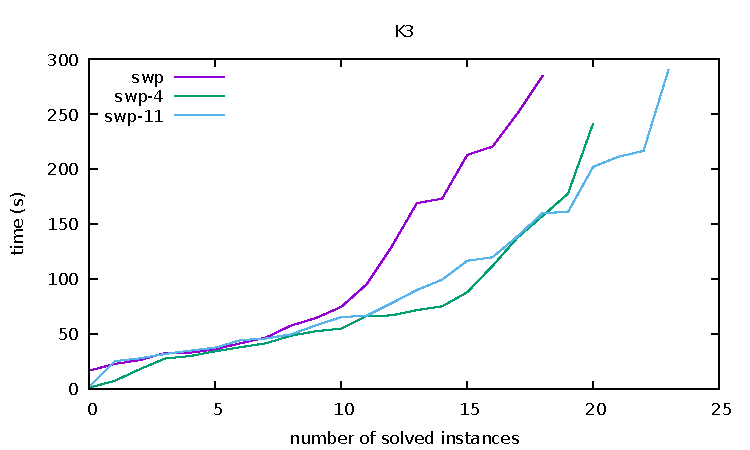
\includegraphics[scale = 0.9]{Parallel/K3/e2.pdf}
\end{frame}
\begin{frame}
\frametitle{5SAT}
    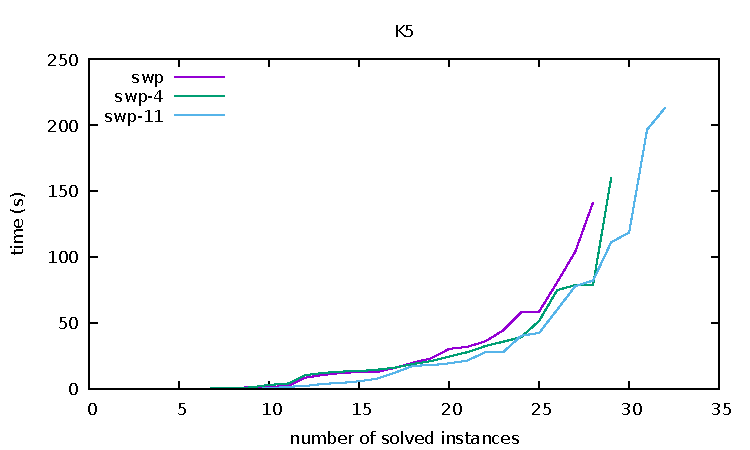
\includegraphics[scale = 0.9]{Parallel/K5/e2.pdf}
\end{frame}
\begin{frame}
\frametitle{7SAT}
  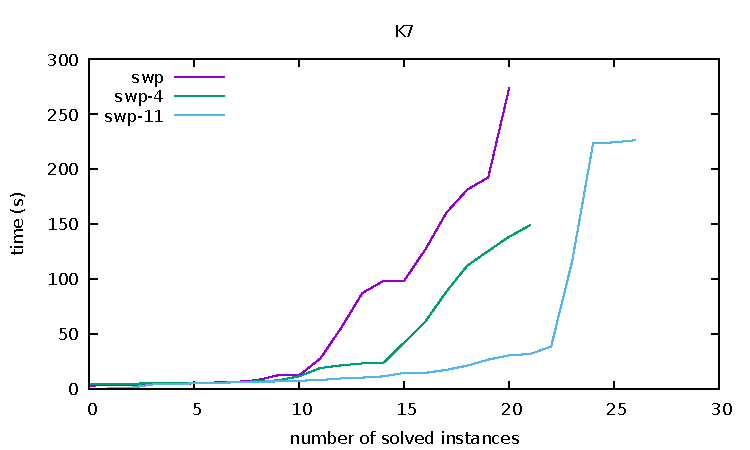
\includegraphics[scale = 0.9]{Parallel/K7/e2.pdf}
\end{frame}
\begin{frame}
\frametitle{Conclusion}
\heading{Our improvement:}
\begin{itemize}
\item a stochastic local search algorithm \emph{swpSAT} with the incorporation of \emph{walkSAT} and \emph{probSAT}
\item different local variants, which get better performance than the \emph{probSAT} algorithm
\item parallel \emph{swpSAT} solver with formula partitioning
\item the formula partitioning information can guide the local search
\end{itemize}
\heading{Further work}
\begin{itemize}
\item use different search strategies
\item use different cooperation strategies
\item use different random generation in local search
\end{itemize}
\end{frame}
\begin{frame}
 \begin{figure}

\includegraphics[scale=0.2]{1/thank-you-for-your-attention-any-questions-78.png}
\end{figure}   
\end{frame}
\end{document}
